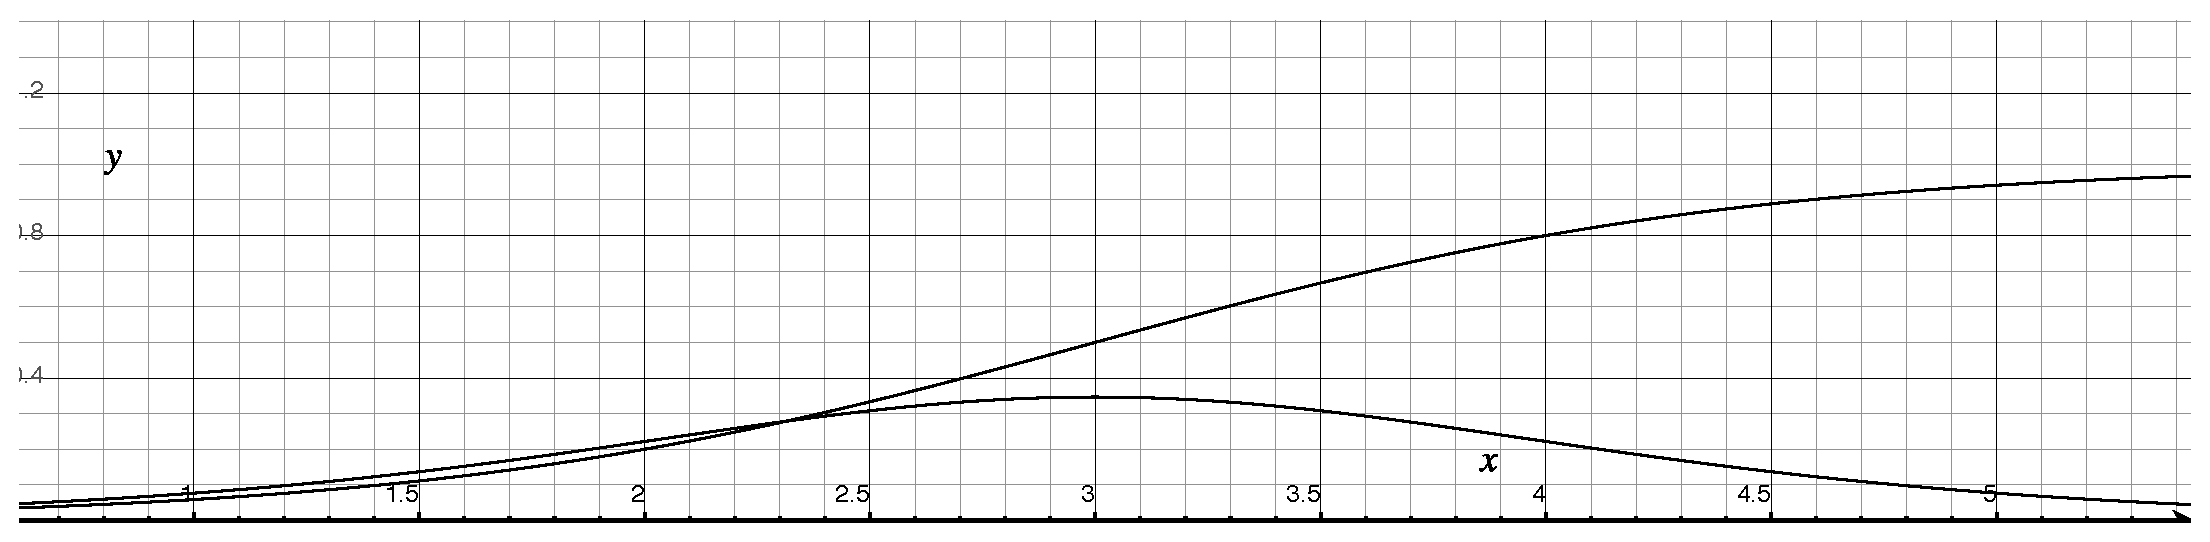
\includegraphics[scale=1.02]{images/F(x)_ext.eps}

% $f(x) = 1-\frac{1}{1+2^{2(x-3)} } $

There is an $F()$ mentioned in the title. 
The rising line in the figure above is the $Function\ F()$ curve provided by the topic, while the other is the $Function\ F$ after differential. We can know that the light color line reached the highest peak of the increase at 3. Therefore, when the second to third and third to fourth exercises are equal and the largest, to get the result of the most points in one more class, we try to set the number of single-subject exercises to 4. 
~\\

\innerblock{Expected Value}{\begin{tikzpicture}
% \node[draw=Orange,fill=Orange,text=G-lig,text width=6cm, rounded corners, text centered] (item1) at (2,4) {item1};

\node[draw=Gray,fill=Gray,text=G-lig,text width=4cm,rounded corners, text centered] (item1) at (7,0) {item1};

\node[draw=Gray,text width=4cm,fill=Gray,rounded corners, text centered, text=FontColor, text=G-lig] (item2) at (17,3) {item2};

\node[text width=4cm,rounded corners, text centered, text=FontColor, text=G-lig] (item3) at (13.5,1.5) {item3};

\node[text width=4cm,rounded corners, text centered, text=FontColor, text=G-lig] (item4) at (13.5,-1.5) {item4};

\node[draw=LightRed,text width=4cm,fill=LightRed,text=G-lig,rounded corners, text centered] (item5) at (17,-3) {item5};

\node[draw=LightRed,text width=4cm,fill=LightRed,text=G-lig,rounded corners, text centered] (item6) at (30.5,1.5) {item6};

\node[draw=LightRed,text width=4cm,fill=LightRed,text=G-lig,rounded corners, text centered] (item7) at (30.5,5.5) {item7};

\node[draw=purple,text width=4cm,fill=purple,text=G-lig,rounded corners, text centered] (item8) at (30.5,-1.5) {item8};

\node[draw=LightRed,text width=4cm,fill=LightRed,text=G-lig,rounded corners, text centered] (item9) at (30.5,-5.5) {item9};

\node[text width=4cm,text=G-lig,rounded corners, text centered] (item10) at (26.25,4.5) {item10};

\node[text width=4cm,text=G-lig,rounded corners, text centered] (item11) at (26.25,2.25) {item11};

\node[text width=4cm,text=G-lig,rounded corners, text centered] (item12) at (26.25,-4.5) {item12};

\node[text width=4cm,text=G-lig,rounded corners, text centered] (item13) at (26.25,-2.25) {item13};

\draw[->,line width=1mm, draw=FontColor,] (item1) to (item2);
\draw[->,line width=1mm,draw=FontColor] (item1) to (item5);
\draw[->,line width=1mm,draw=FontColor] (item2) to (item6);
\draw[->,line width=1mm,draw=FontColor] (item2) to (item7);
\draw[->,line width=1mm,draw=FontColor] (item5) to (item8);
\draw[->,line width=1mm,draw=FontColor] (item5) to (item9);

\end{tikzpicture}

}

$ R \% \times Points \times [1 - Q\% \times(1 - K\%)] $

% \hspace{2.2cm}
% \transparent{0.6}

In terms of code, it can be implemented in a way similar to random algorithms. Specifically, we will list all possible courses for each day first, and then we can use the number to fill in each semester. Because there are many restrictions when filling the course, we will pop out the course when it doesn't meet the requirements. 
~\\

The expectation of using random as the basis for course selection is about 60. After repeating it one hundred times, it can reach the peak of 99.
~\\

\includegraphics[scale=1.3]{images/1000times.png}
\includegraphics[scale=1.3]{images/10000times.png}

Figure 1 above shows the point distribution diagram of randomly extracting all legally selected courses 1000 times; Figure 2 shows the point distribution diagram randomly extracting 10000 times. From the two charts,  the maximum value can be found from this search, which is 95.13.